\documentclass[10pt]{beamer}
%\usetheme{Boadilla}
%\usecolortheme{beaver}
%\usepackage[latin1]{inputenc}
\usefonttheme[onlymath]{serif}
\usepackage{amsmath}%
\usepackage{amsthm}%
\usepackage{amsfonts}%
\usepackage{amssymb}%
\usepackage{tikz}
\usepackage[english]{babel}
\usepackage{amsmath, amssymb, amsthm}
\usepackage{verbatim}
\usepackage{mathrsfs}
%\usepackage{epstopdf}
\usepackage{graphicx}
\newcommand{\mrel}{\mathrel{\bigcirc}}
%\usepackage[onehalfspacing]{setspace}
%\setbeamertemplate{footline}[frame number]
\DeclareMathOperator*{\Bigcdot}{\scalerel*{\cdot}{\bigodot}}
% Macros
\def\a{\alpha} \def\b{\beta} \def\c{\gamma} \def\d{\delta} \def\r{\rho}
\def\e{\epsilon} \def\ve{\varebsilon} \def\k{\kappa} \def\p{\pi} \def\th{\theta}
\def\l{\lambda} \def\m{\mu} \def\s{\sigma} \def\t{\tau} \def\w{\omega} \def\z{\zeta}
\def\D{\Delta} \def\G{\Gamma} \def\W{\Omega} \def\P{\Phi} \def\L{\Lambda}
\def\bdm{\begin{displaymath}} \def\edm{\end{displaymath}}
\def\bni{\begin{itemize}} \def\ei{\end{itemize}}
\def\bnen{\begin{enumerate}} \def\een{\end{enumerate}}
\def\fa{\forall}
\def\be{\begin{equation}} \def\ee{\end{equation}}
\def\fn{\footnote} \def\bn{\begin} \def\nit{\noindent}
\def\iff{\textit{~if and only if~~}}

% THEOREMS -------------------------------------------------------
\newtheorem{thm}{Theorem}%[section]
\newtheorem{cor}[thm]{Corollary}
\newtheorem{lem}[thm]{Lemma}
\newtheorem{prop}[thm]{Proposition}
\newtheorem{claim}{Claim}
\theoremstyle{definition}
%\newtheorem{defn}[thm]{Definition}
\theoremstyle{remark}
\newtheorem{rem}[thm]{Remark}
%%\numberwithin{equation}{section}  
 
\newcommand{\N}{\mathbb{N}}
\newcommand{\Z}{\mathbb{Z}}
\newcommand{\R}{\mathbb{R}}
\newcommand{\ls}{\left\{}
\newcommand{\rs}{\right\}}


\title{A Network Model for \\Dynamic Textual Communications \\with Application to
	Government Email Corpora}
\author{
Bomin Kim\textsuperscript{1}\and
\quad Aaron Schein\textsuperscript{3}\and\\
		Bruce Desmarais \textsuperscript{1}\and Hanna Wallach\textsuperscript{2,3}}
\institute{\textsuperscript{1} The Pennsylvania State University \and \textsuperscript{2} Microsoft Research NYC \and \textsuperscript{3} University of Massachusetts Amherst}
\begin{document}
 
\begin{frame}
  \titlepage
\end{frame}

\begin{frame}{Interaction-Partitioned Topic Model (IPTM)}
	\bni
	\item Probablistic model for time-stamped textual communications \\
	(e.g. emails, cosponsorship of bills, international sanctions)		\vspace{0.2cm}
	\item Integration of two generative models:\\
	 - Latent Dirichlet allocation (LDA) for topic-based contents\\
	 - Dynamic exponential random graph model (ERGM) for ties\\
\vspace{0.2cm}
	\item IPTM assigns each topic to an ``interaction pattern," which is governed by a set of dynamic network features
	\ei
		\vspace{0.4cm}
\centering \large\textit{``who communicates with whom about what, and when?"}
\end{frame}

\begin{frame}{Content Generating Process: LDA (Blei et al., 2003)}
\bni 
\item For each topic $k =1,...,K:$\vspace{0.2cm}
	\begin{itemize}
		\item[1.] Topic-word distribution {$\boldsymbol{\phi}^{(k)} \sim \mbox{Dirichlet}(\beta, \bf u)$}\\
		- A topic $k$ is characterized by a discrete distribution over $V$ word types with probability vector $\boldsymbol{\phi}^{(k)}$. \vspace{0.2cm}
		\item[2.] Topic-IP distribution $c_k\sim \mbox{Uniform}(1, C)$\\
		- Each topic is associated with a single interaction pattern.			
		\end{itemize}\vspace{0.4cm}
\item For each document $d =1,...,D:$ \vspace{0.2cm}
	\begin{itemize}
\item[3-1.] Document-topic distribution $\boldsymbol{\theta}^{(d)}\sim \mbox{Dirichlet}(\alpha, \boldsymbol{m})$\\
- A document $d$ is characterized by a discrete distribution over $K$ topics with probability vector $\boldsymbol{\theta}^{(d)}$. \vspace{0.2cm}
		\item[3-2.] For each word in a document $n=1$ to $N^{(d)}$:
		\begin{itemize}
			\item[(a)] Choose a topic $z_n^{(d)} \sim \mbox{Multinomial}(\boldsymbol{\theta}^{(d)})$
			\item[(b)] Choose a word $w_n^{(d)} \sim\mbox{Multinomial} (\boldsymbol{\phi}^{(z_n^{(d)})})$
		\end{itemize}
	\end{itemize}
\ei	
\end{frame}


\begin{frame}{Dynamic Network Features (Perry and Wolfe, 2012)}
	 \begin{figure}
	 	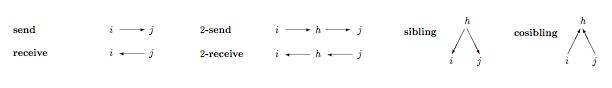
\includegraphics[width=0.85\textwidth]{PerryWolfeimage.jpeg}
	 \end{figure}	
	 
\end{frame}


\begin{frame}{Tie Generating Process}
\end{frame}
\begin{frame}{Inference - Pseudocode}
\end{frame}

\begin{frame}{Data: North Carolina Dare county email data}
 \bni \item $D = 1456$ emails between $A = 27$ county government managers, covering 2 month periods (October 1 - November 30) in 2013\ei
 \begin{figure}
 	\includegraphics[width=0.55\textwidth]{Dare.png}
 \end{figure}	
\end{frame}

\begin{frame}{Effect of Hurricane Sandy}
\end{frame}

\begin{frame}{IPTM Result}
\end{frame}

\begin{frame}{Conclusion}
 \bni
 \item Joint modeling of ties (sender, receiver, time) and contents
 	\vspace{0.4cm}
 \item Allowance of multicast -- multiple senders and/or receivers
 	\vspace{0.4cm}
 \item Possible application to 
 \ei
\end{frame}
\end{document}